\documentclass[10pt,conference,letterpaper]{IEEEtran}
\usepackage{amsmath,amssymb}
\usepackage{graphicx}
\usepackage{booktabs}
\usepackage{microtype}
\usepackage{url}
\usepackage[hidelinks]{hyperref}
\hypersetup{
  pdfauthor={Le Dong},
  pdftitle={Deterministic Target-Conditioned Gaussian-Process Optimization for Small-Budget Electromagnetic Design}
}
\setlength{\textfloatsep}{6pt plus 1pt minus 2pt}
\setlength{\floatsep}{6pt plus 1pt minus 2pt}

\title{Deterministic Target-Conditioned Gaussian-Process Optimization for Small-Budget Electromagnetic Design}
\author{\IEEEauthorblockN{Le Dong}
\IEEEauthorblockA{\textit{School of Electrical Engineering}\\
\textit{Xi'an Jiaotong University}\\
Xi'an, Shaanxi 710049, China\\
\texttt{leroi\_2024@stu.xjtu.edu.cn}}}

\begin{document}
\maketitle

\begin{abstract}
Electromagnetic component design often requires a target response within a tolerance band while minimizing resistance or loss with few model evaluations. We develop a deterministic, target-conditioned Gaussian-process (GP) workflow that starts at the domain center and fits hyperparameters from fixed initial points. Sampling first seeks feasibility, then follows constrained expected improvement (cEI) until a relative-cEI stopping criterion is met, followed by 10 verification evaluations. With the workflow settings fixed on 14 development targets, all 73 held-out targets of a 1,110-design air-core coil benchmark reach the exact global optimum at a mean cost of 21.81 evaluations. Six-point random initialization under the same fitting and stopping rules recovers 859 of 870 target-seed optima. On an eight-dimensional wireless power transfer (WPT) benchmark, both the proposed workflow and budget-matched conventional cEI find feasible designs for all 21 targets, compared with 10/21 for Sobol search. Adaptive stopping saves 29.9\% of evaluations relative to a fixed budget of 50, with a 3.75\% increase in mean DC resistance. In an 85~kHz 3-D Ansys Maxwell eddy-current test at 1000~nH, the automatic run stops at 30 total evaluations and returns an AC resistance of $383.68~\mathrm{m}\Omega$, compared with $389.54~\mathrm{m}\Omega$ for the matched baseline.
\end{abstract}

\begin{IEEEkeywords}
Adaptive stopping, Bayesian optimization, constrained expected improvement, electromagnetic design, surrogate modeling.
\end{IEEEkeywords}

\section{Introduction}
Electromagnetic design frequently requires matching a target physical response $g_t$ within a strict relative tolerance band $\epsilon$ while minimizing a competing objective. For a forward model returning a constrained response $g(x)$ and scalar objective $J(x)$ over design space $\mathcal X$, the target-conditioned optimization problem is
\begin{equation}
 \min_{x\in\mathcal X}J(x)\quad\mathrm{s.t.}\quad
 \frac{|g(x)-g_t|}{|g_t|}\leq\epsilon .
 \label{eq:problem}
\end{equation}
Here, $J(x)$ may represent winding resistance or a scalarized combination of loss, mass, and thermal rise. When each evaluation requires a finite-element simulation or hardware measurement, only a small number of designs may be affordable. The optimizer must use these evaluations to find the feasible region and improve the objective before deciding when to stop.

Gaussian-process Bayesian optimization and constrained expected improvement (cEI) \cite{gardner} provide established tools for this problem. Electromagnetic applications include antenna optimization \cite{liu2014,wu2024} and WPT coil design \cite{sim2023}. Regret-based stopping criteria \cite{ishibashi2023} have also been studied in general BO. However, initialization, hyperparameter fitting, and stopping decisions remain important practical choices when electromagnetic optimization is limited to a few dozen model evaluations.

We examine these choices in three stages: 1) compare surrogate families and acquisition functions on an exhaustive 1,110-design coil domain; 2) develop deterministic initialization and GP fitting with adaptive stopping; and 3) evaluate the resulting workflow on held-out 2-D targets, an eight-dimensional WPT problem, and a 3-D Ansys Maxwell eddy-current solver.

\section{Models and Optimization Method}
\subsection{Two-Dimensional Coil Model}
The first benchmark describes a multilayer air-core coil by radial layers $T\in\{1,\ldots,10\}$ and turns per layer $n\in\{20,\ldots,130\}$. With wire diameter $d=0.68$~mm, pitch $p=1.05d$, inner diameter $D_0=80$~mm, mean diameter $D=D_0+Tp$, height $H=np$, radial thickness $C=Tp$, total turns $N=Tn$, and resistivity $\rho=1.851\times10^{-5}~\Omega\!\cdot\!\mathrm{mm}$, the analytical model is
\begin{equation}
 L=\frac{8\times10^{-6}N^2D^2}{3D+9H+10C}\ \mathrm{mH},\qquad
 R=\frac{4\rho ND}{d^2}\ \Omega.
 \label{eq:coil}
\end{equation}
Full enumeration of the 1,110 integer designs provides the exact global optimum $R_{\text{exhaustive}}$ for each integer target $L_t=1,\ldots,87$~mH. For feasible designs, we measure the relative resistance excess $r=R/R_{\text{exhaustive}}-1$ and report bounded loss $u=r/(1+r)\in[0,1)$. Infeasible designs receive $u=1$.

\subsection{Reusable-Surrogate Screening}
Before target-specific optimization, we compare Gaussian processes (GPs) and deep ensembles (DEs) under a shared $B=17+10=27$ protocol. Both families model $L$ and $R$ independently: the GP baseline fits one Gaussian process per response, whereas the DE fits a 10-member ensemble of single-output multilayer perceptrons (hidden layers of 16 and 8 ReLU units) to each response.

Each surrogate is built from 17 target-agnostic observations and reused across all 87 targets. Random policies draw all 17 points uniformly with fixed seeds; active policies start from the same first six points, then acquire 11 more by maximizing equally weighted, scale-normalized uncertainty in $L$ and $R$. For each target $L_t$, the fitted surrogates rank the remaining 1,093 designs by predicted feasibility and resistance. The top 10 are evaluated, and the lowest-resistance feasible design among these 10 is returned.

As shown in Fig.~\ref{fig:surrogates}, active uncertainty sampling improves both model families across the 870 target-seed cases. For the GP, it raises feasibility from 99.89\% to 100\% and exact optimum recovery from 695 to 740, and cuts all-case mean bounded loss by 57.9\% (from 0.00682 to 0.00287). For the DEs, active sampling raises exact recovery from 274 to 651 and reduces all-case mean loss from 0.310 to 0.104. Because the GP outperforms the DE on every aggregate metric including a mean loss roughly 36$\times$ lower, we use GP surrogates in the target-conditioned study that follows.
\begin{figure}[!t]
 \centering
 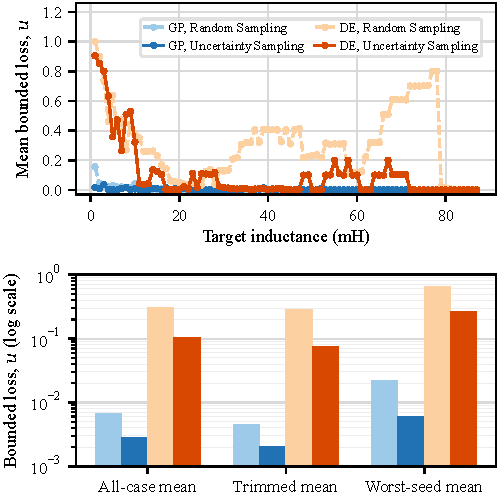
\includegraphics[width=0.98\columnwidth]{../figures/fig01_surrogate_comparison.pdf}
 \caption{Matched reusable-surrogate screen at nominal per-target $B=27$. Both model families use 17 model-building observations and 10 target-specific final evaluations. Lower bounded loss is better.}
 \label{fig:surrogates}
\end{figure}

\subsection{Direct-Search Reference}
As a direct-search reference, we use simulated annealing (SA) \cite{kirkpatrick}, which searches the integer domain with cached evaluations and stops after five cycles without a 1\% improvement in feasible resistance. SA and the reusable active GP use the same $\pm2.5\%$ feasibility band and 10 seeds. After dropping the best and worst seed at each target, the trimmed mean bounded loss is 0.00205 for GP and 0.0451 for SA (Fig.~\ref{fig:gp-sa}), at 27 nominal evaluations for GP and a trimmed mean of 92.1 for SA. The GP's 17 model-building observations serve all 87 targets, whereas SA starts a separate search for each; thus, the nominal per-target budgets are not equivalent to the amortized costs across all targets. The reusable GP nevertheless misses 130 of 870 exact optima. We next test whether conditioning sequential acquisition on $L_t$ improves recovery at the same nominal budget ($B=27$).

\begin{figure}[!t]
 \centering
 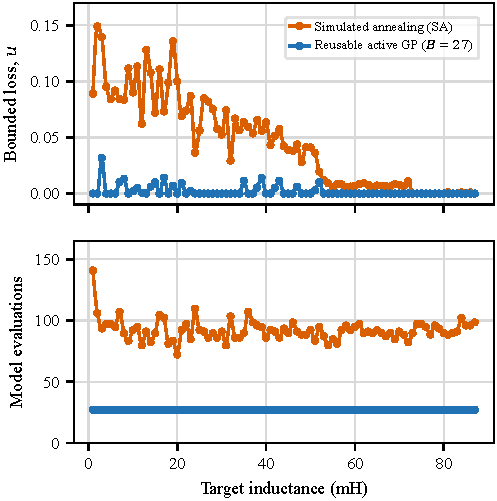
\includegraphics[width=0.98\columnwidth]{../figures/fig02_gp_vs_sa.pdf}
 \caption{Reusable active GP versus direct SA. The upper panel reports targetwise-trimmed bounded loss and the lower panel reports forward-model evaluations.}
 \label{fig:gp-sa}
\end{figure}

\subsection{Target-Conditioned Acquisition}
We model $L$ and $R$ with independent GPs and additive white-noise terms. The 2-D benchmark uses RBF kernels; WPT uses isotropic Mat\'ern-$5/2$ kernels, allowing less smooth functions and sharing one length scale across normalized coordinates to limit hyperparameter count under small evaluation budgets \cite[ch.~4]{rasmussen}. For target $L_t$ and tolerance $\epsilon=0.025$, we compute the probability of satisfying the inductance constraint as
\begin{equation}
 \begin{aligned}
 p_F(x) &= \Phi(z_+(x)) - \Phi(z_-(x)),\\
 z_{\pm}(x) &= \frac{L_t(1 \pm \epsilon) - \mu_L(x)}{\sigma_L(x)},
 \end{aligned}
 \label{eq:pf}
\end{equation}
where $\mu_L(x)$ and $\sigma_L(x)$ are the posterior mean and standard deviation, and $\Phi(\cdot)$ is the standard normal cumulative distribution function. Here, $L$ denotes the constrained inductive response, including mutual inductance $M$ in WPT.

Once a feasible design has been observed, we select the next design by maximizing the constrained expected improvement (cEI) acquisition function $a_{\mathrm{cEI}}(x)=p_F(x)\mathrm{EI}_R(x)$, where
\begin{equation}
 \begin{aligned}
 \mathrm{EI}_R(x)&=\sigma_R(x)\bigl[z_R(x)\Phi(z_R(x))+\phi(z_R(x))\bigr],\\
 z_R(x)&=\frac{R^*-\mu_R(x)}{\sigma_R(x)}.
 \end{aligned}
 \label{eq:ei}
\end{equation}
Here, $\mu_R(x)$ and $\sigma_R(x)$ are the resistance posterior mean and standard deviation. $\mathrm{EI}_R(x)$ represents the expected positive improvement over the best observed feasible resistance $R^*$, and $\phi(\cdot)$ is the standard normal density. At zero posterior variance, $\mathrm{EI}_R(x)=\max\{R^*-\mu_R(x),0\}$.

Across 10 seeds and 87 targets at $B=6+11+10=27$ (Fig.~\ref{fig:acquisition}), cEI recovers 867/870 exhaustive optima with mean bounded loss 0.000161. Constrained lower confidence bound (cLCB) recovers 829 with mean loss 0.00274, while integrated variance reduction (IVR) recovers 827 with mean loss 0.000819. cEI leads on both measures. The two extra recoveries obtained by cLCB over IVR come with larger losses in the remaining cases.

\begin{figure}[!t]
 \centering
 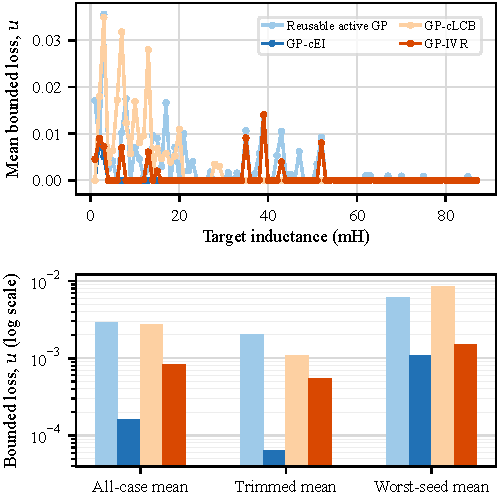
\includegraphics[width=0.98\columnwidth]{../figures/fig03_acquisition_comparison.pdf}
 \caption{Matched target-conditioned acquisition comparison at $B=27$ over 10 seeds and 87 targets. Lower bounded loss is better.}
 \label{fig:acquisition}
\end{figure}

\subsection{Deterministic Feasibility Discovery and Fitting}
The fixed-budget cEI baseline recovers 867 of 870 optima, but its trajectories still depend on random initialization and stochastic GP fitting. To obtain reproducible small-budget searches, each run instead begins at the normalized domain center. With only one observation, maximizing $p_F$ alone can focus sampling too narrowly. Before feasibility is observed, we therefore use
\begin{equation}
 a_F(x)=\omega\,\operatorname{norm}(p_F(x))
       +(1-\omega)\,\operatorname{norm}(\sigma_L(x)),
 \label{eq:start}
\end{equation}
where $\omega\in[0,1]$ is the feasibility weight and $\operatorname{norm}(\cdot)$ min--max normalizes values over the unobserved candidate set. After the first feasible design is found, acquisition switches to cEI.

We hold kernel hyperparameters fixed for the first three observations. From the fourth onward, we maximize marginal likelihood for each GP using L-BFGS-B from $K$ fixed starting points: the initial hyperparameters and $K-1$ Halton points in the bounded log-hyperparameter domain. Retaining the highest-likelihood solution among these $K$ fits removes random restarts during both feasibility discovery and cEI sampling.

Let $R_k^*$ be the best feasible resistance after refit $k$. The unobserved candidate pool $\mathcal C_k$ consists of the remaining integer designs in the 2-D benchmark or deterministic Sobol candidates in WPT. We monitor the maximum relative cEI
\begin{equation}
 \rho_k=\max_{x\in\mathcal C_k}
 \frac{p_F(x)\mathrm{EI}_R(x)}{R_k^*}.
 \label{eq:stop}
\end{equation}
For a $d$-dimensional problem, adaptive sampling ends only after at least $N_{\min}=2d+1$ model-building observations and $P$ consecutive refits satisfying $\rho_k\leq\delta$, where $\delta$ is the relative-cEI threshold and $P$ is the stopping patience. For final verification, 10 unobserved candidates are ranked by $p_F(x)\exp[-\operatorname{norm}(\mu_R(x))]$, favoring high feasibility probability and low predicted resistance without an objective-uncertainty exploration bonus. These candidates are evaluated as a fixed batch, and the lowest-resistance feasible design among all observations is returned.

The reported evaluation count includes initialization, sequential sampling, and the final verification batch.

\section{Experimental Protocol}
We evaluate the 2-D benchmark at all 87 integer targets from 1 to 87~mH, using 10 fixed seeds for each stochastic method (870 target-seed cases). The fixed-budget acquisition comparison allocates six initial observations, 11 sequential acquisitions, and 10 final evaluations to each method. Losses and exact-recovery counts are computed against exhaustive enumeration.

We screened the feasibility weight on 10 targets spanning the domain, then examined the random-six cEI misses at 2--5~mH. Using the resulting 14-target development set, we selected $\omega=0.75$, $K=5$, $\delta=0.01$, and $P=3$, and fixed these settings before evaluating the 73 held-out targets. The three-observation fitting warmup and 10-point verification batch are fixed protocol choices. Replays with different seed labels check that the deterministic implementation ignores the seed input.

For numerical WPT, we use 21 targets from 1000 to 2000~nH in 50~nH steps. Comparators are conventional cEI, a center-start $p_F$-then-cEI control, Sobol search, and a fixed 50-evaluation control. Conventional cEI and Sobol search receive the automatic run's realized budget at each target. To contain the cost of 8-D comparisons, conventional cEI uses six fixed Sobol initial points in both the analytical and Maxwell tests instead of 10-seed replication. Random-start sensitivity is nevertheless tested at 1500~nH by running the otherwise unchanged automatic workflow from six uniformly random points for each of 10 fixed seeds. In a separate 1000~nH test with an 85~kHz Maxwell 3-D eddy-current solver, the automatic workflow establishes a budget of 20 model-building and 10 verification evaluations; conventional cEI receives the same budget. The responses are mutual inductance and the sum of the impedance matrix's Tx/Rx AC self-resistances.

The companion repository contains raw records, hyperparameters, candidate histories, figure scripts, and checks of the reported budgets and outcomes. For the analytical benchmarks, each optimizer accesses the equations through the same forward-model interface.

\section{Two-Dimensional Validation}
All 73 held-out targets reach the exhaustive optimum, and every run stops naturally (Table~\ref{tab:two-d}). The mean total cost is 21.81 evaluations, with a median of 22 and a range of 19--25. Since model building takes 9--15 evaluations, the $2d+1=5$ minimum never determines the stopping point in these 2-D runs.

To examine sensitivity to the starting policy under deterministic fitting, we also use six random initial points while retaining the development-set values of $\omega$, $K$, $\delta$, and $P$ and the 10-point verification batch. Neither automatic policy has an evaluation cap. Random-six recovers 859/870 optima, with seed-dependent results at eight targets; all runs stop naturally, using 18--31 evaluations. Paired by target, the center-start policy wins 11 cases, ties 859, and loses none. Mean costs are 22.60 for random-six and 21.93 for the center policy across all 87 targets.

At the stopping point, posterior coverage within the feasible region is 80.8\%/96.5\% at $1\sigma/2\sigma$ for $L$ and 82.1\%/96.3\% for $R$ across the held-out targets.

\begin{table}[!t]
\caption{Optimization results on the 2-D coil benchmark.}
\label{tab:two-d}
\centering
\footnotesize
\begin{tabular}{@{}lrrr@{}}
\toprule
Configuration & Cases & Exact & Mean evaluations \\
\midrule
cEI, fixed $6+11+10$ & 870 & 867 & 27.00 \\
Automatic, development & 14 & 14 & 22.57 \\
Automatic, held out & 73 & 73 & 21.81 \\
Random-six + same stopping & 870 & 859 & 22.60 \\
Deterministic center (unique) & 87 & 87 & 21.93 \\
\bottomrule
\end{tabular}
\end{table}

\section{Application to Eight-Dimensional WPT Coil Design}
\subsection{Controlled Black-Box Benchmark}
The WPT model of Asadi and Abazari has eight geometry variables and six pose variables \cite{asadi2025}. We fix translation at $(0,0,70)$~mm and all rotations at zero, then optimize polygon side count $n_s\in\{4,\ldots,10\}$, turn count $n_t\in\{5,\ldots,15\}$, spacing $s\in[1,3]$~mm, and inner radius $r_i\in[30,80]$~mm for each coil. This leaves eight variables, with integer counts and continuous dimensions.

The constraint is $|M(x)-M_t|/M_t\leq0.025$. Total DC resistance is computed from polygonal conductor centerline length,
\begin{equation}
 R=\frac{\rho_{\mathrm{Cu}}}{A}\sum_{q\in\{t,r\}}\sum_{k=0}^{n_{t,q}-1}
 2n_{s,q}r_{q,k}\sin(\pi/n_{s,q}),
 \label{eq:wpt-r}
\end{equation}
where $r_{q,k}=r_{i,q}+k(s_q+w)$, $w=0.68$~mm, $A=\pi(w/2)^2$, and $\rho_{\mathrm{Cu}}=1.851\times10^{-5}~\Omega\!\cdot\!\mathrm{mm}$. Leads are excluded. Mutual inductance is computed using the partial-inductance model in \cite{asadi2025}.

Both responses are presented to the optimizer as black-box outputs and learned by separate GPs. This provides a controlled comparison under equal evaluation budgets; the subsequent Maxwell experiment tests direct operation with a field solver.

Starting from the normalized center, we select candidates from consecutive blocks of one unscrambled Sobol sequence. With the isotropic Mat\'ern-$5/2$ kernel, we retain $\omega=0.75$, $K=5$, $\delta=0.01$, $P=3$, and 10 verification evaluations, testing transfer of the workflow settings without retuning. The dimensional rule gives $N_{\min}=17$. Automatic runs have no evaluation cap. A separate fixed-budget control uses 40 model-building and 10 verification evaluations.

\begin{figure}[!t]
 \centering
 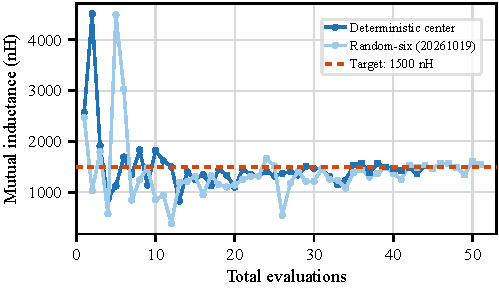
\includegraphics[width=0.98\columnwidth]{../figures/fig04_initialization_reliability.pdf}
 \caption{WPT trajectories at 1500~nH. Squares mark final verification; the dashed line marks the target.}
 \label{fig:reliability}
\end{figure}
\subsection{Results}
Automatic and conventional cEI both find feasible designs for all 21 targets, as does the center-start $p_F$-then-cEI control, compared with 10/21 for Sobol search. Mean resistances for automatic and conventional cEI are $314.9$ and $315.5~\mathrm{m}\Omega$ (Table~\ref{tab:wpt}). Automatic cEI wins eight targets, ties four, and loses nine (paired Wilcoxon $p=0.981$), with no clear resistance advantage on this set.

Table~\ref{tab:wpt} lists five representative targets and the 21-target summary, where $B_s$ is the automatic evaluation count, $R_s$ the returned resistance, and $R_{50}$ the resistance under the fixed 50-evaluation control.

\begin{table}[!t]
\caption{Optimization results on the 8-D WPT benchmark.}
\label{tab:wpt}
\centering
\footnotesize
\begin{tabular}{@{}rrrrrr@{}}
\toprule
$M_t$ (nH) & $B_s$ & \multicolumn{4}{c}{Resistance (m$\Omega$)} \\
\cmidrule(lr){3-6}
& & $R_s$ & $R_{50}$ & Conv. & Sobol \\
\midrule
1000 & 33 & 259.7 & 259.7 & 259.7 & -- \\
1250 & 34 & 291.5 & 280.3 & 340.4 & -- \\
1500 & 44 & 305.8 & 305.8 & 305.6 & 343.9 \\
1750 & 27 & 332.5 & 324.9 & 332.5 & -- \\
2000 & 27 & 377.0 & 343.7 & 371.1 & 422.8 \\
\midrule
Mean (21) & 35.05 & 314.9 & 303.5 & 315.5 & -- \\
Feasible & -- & 21/21 & 21/21 & 21/21 & 10/21 \\
\bottomrule
\end{tabular}
\end{table}

All 21 runs stop naturally, including four at the $N_{\min}=17$ minimum. Relative to the fixed $B=50$ control, adaptive stopping reduces the mean count to 35.05 evaluations (29.9\% fewer), with 3.75\% higher mean resistance.

At 1500~nH, feasibility is first reached at evaluation 12 and model building stops after 34 evaluations. After 10 verification evaluations, the returned design has $M=1466.48$~nH and $R=305.77~\mathrm{m}\Omega$, only 3.98~nH above the lower bound. As Fig.~\ref{fig:reliability} illustrates, the random-six run requiring the most evaluations among the 10 seeds (seed 20261019) uses seven more evaluations than the deterministic run (51 versus 44, or 15.9\% more) and returns a higher resistance ($309.57$ versus $305.77~\mathrm{m}\Omega$). The selected deterministic Tx/Rx coils have 9/7 sides, 7/7 turns, 1.741/2.709~mm spacing, and 61.724/61.007~mm inner radii (Fig.~\ref{fig:wpt-geometry}).

\subsection{Field-Solver Application Check}
With Maxwell at 1000~nH, the automatic workflow stops after 20 model-building evaluations and performs 10 verification evaluations. Each coil is modeled as a continuous solid-copper spiral with interior field solution enabled; adaptive solves use a 2\% error target, 30\% refinement, and two to four passes. We match the automatic budget with six fixed Sobol points, 14 conventional-cEI evaluations, and 10 verification evaluations. Both methods find feasible designs: the automatic run returns $M=998.929$~nH and $R_{\mathrm{AC,Tx}}+R_{\mathrm{AC,Rx}}=383.68~\mathrm{m}\Omega$, compared with $1016.402$~nH and $389.54~\mathrm{m}\Omega$ for the baseline. It obtains seven feasible observations versus three, although the baseline reaches feasibility earlier (evaluation 6 versus 12). The returned AC resistance is 1.50\% lower for the automatic run. This experiment demonstrates that the workflow can operate directly with a 3-D field solver under the same optimization settings.

\begin{figure}[!t]
 \centering
 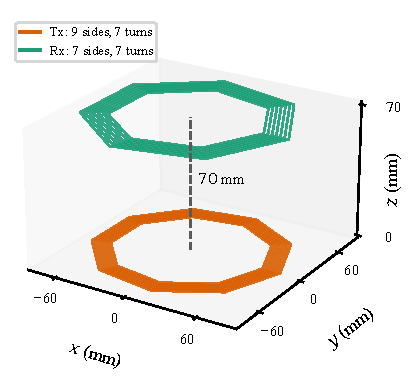
\includegraphics[width=0.82\columnwidth]{../figures/fig05_numerical_wpt_geometry.pdf}
 \caption{Selected nominal-pose 1500~nH design. The aligned transmitter and receiver planes are separated by 70~mm.}
 \label{fig:wpt-geometry}
\end{figure}

Fig.~\ref{fig:maxwell-geometry} shows the automatic run's selected Maxwell geometry from evaluation 25, in the final verification batch.
\begin{figure}[!t]
 \centering
 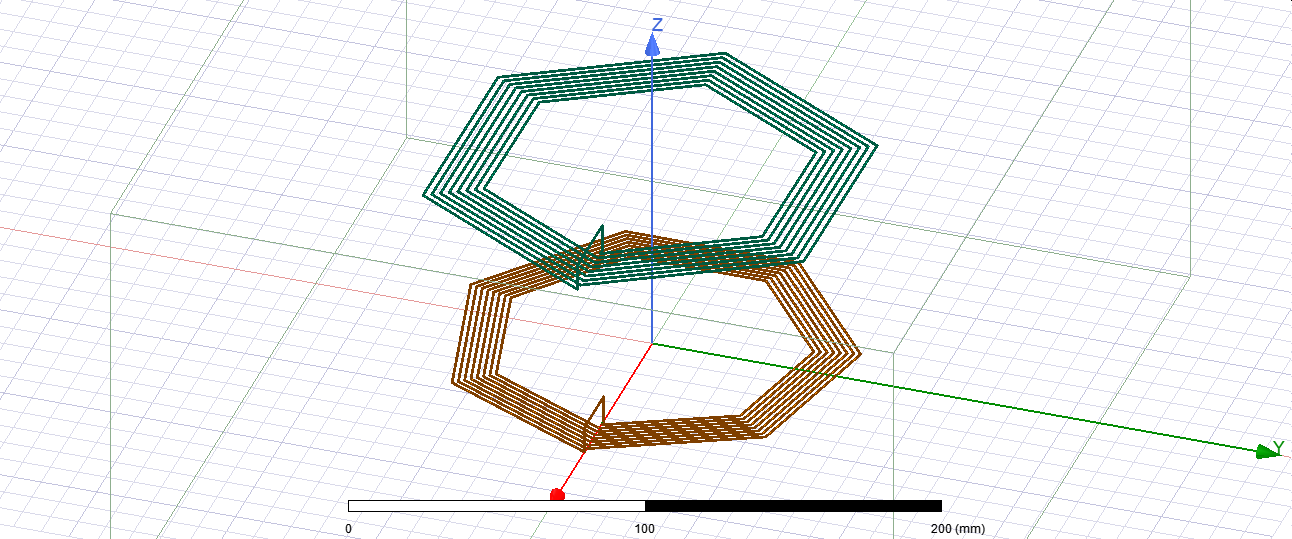
\includegraphics[width=0.98\columnwidth]{../figures/fig06_maxwell_selected_geometry.png}
 \caption{Selected Maxwell geometry at evaluation 25: seven-sided Tx (orange), six-sided Rx (green), eight turns each, separated by 70~mm.}
 \label{fig:maxwell-geometry}
\end{figure}

\section{Discussion and Conclusion}
Center initialization and fixed GP fitting remove seed dependence from the implemented search. Settings selected on 14 targets recover all 73 held-out optima. On 21 WPT targets, automatic and conventional cEI both achieve full feasibility; adaptive stopping saves evaluations at a measurable resistance cost relative to the fixed 50-evaluation control, while center initialization eliminates initialization-seed variability. The 1000~nH Maxwell test extends validation from analytical models to eddy-current simulation without retuning the core optimization settings.

The workflow settings were selected empirically on the 14-target development set. Validation covers analytical coils, fixed-pose numerical WPT, and one Maxwell target; broader field-solver tests, hardware measurements, and coil misalignment remain future work. Code, data, and validation scripts are publicly available in the \href{https://github.com/le-dong-xjtu/reproducible-target-informed-gp}{companion GitHub repository}.

\begin{thebibliography}{00}
\bibitem{gardner} J. Gardner, M. Kusner, Z. Xu, K. Weinberger, and J. Cunningham, ``Bayesian optimization with inequality constraints,'' in \emph{Proc. ICML}, vol. 32, 2014, pp. 937--945.
\bibitem{liu2014} B. Liu \emph{et al.}, ``An efficient method for antenna design optimization based on evolutionary computation and machine learning techniques,'' \emph{IEEE Trans. Antennas Propag.}, vol. 62, no. 1, pp. 7--18, 2014.
\bibitem{wu2024} Q. Wu, W. Chen, C. Yu, H. Wang, and W. Hong, ``Machine-learning-assisted optimization for antenna geometry design,'' \emph{IEEE Trans. Antennas Propag.}, vol. 72, no. 3, pp. 2083--2095, 2024, doi: 10.1109/TAP.2023.3346493.
\bibitem{sim2023} B. Sim \emph{et al.}, ``Bayesian optimization based fast and accurate wireless power transfer system coil optimization for high efficiency,'' in \emph{Proc. IEEE WPTCE}, 2023, pp. 1--5, doi: 10.1109/WPTCE56855.2023.10215668.
\bibitem{ishibashi2023} H. Ishibashi, M. Karasuyama, I. Takeuchi, and H. Hino, ``A stopping criterion for Bayesian optimization by the gap of expected minimum simple regrets,'' in \emph{Proc. AISTATS}, vol. 206, 2023, pp. 6463--6497.
\bibitem{kirkpatrick} S. Kirkpatrick, C. D. Gelatt, Jr., and M. P. Vecchi, ``Optimization by simulated annealing,'' \emph{Science}, vol. 220, no. 4598, pp. 671--680, 1983.
\bibitem{rasmussen} C. E. Rasmussen and C. K. I. Williams, \emph{Gaussian Processes for Machine Learning}. MIT Press, 2006.
\bibitem{asadi2025} M. Asadi and A. M. Abazari, ``A data-driven model to predict mutual inductance between planar coils with arbitrary specifications and positions,'' \emph{IET Electr. Power Appl.}, vol. 19, Art. no. e70015, 2025, doi: 10.1049/elp2.70015.
\end{thebibliography}

\end{document}
